%-----------------------------------------------
% Template para criação de resumos de projectos/dissertação
% jlopes AT fe.up.pt,   Fri Jul  3 11:08:59 2009
%-----------------------------------------------

\documentclass[9pt,a4paper]{extarticle}

%% English version: comment first, uncomment second
\usepackage[portuguese]{babel}  % Portuguese
%\usepackage[english]{babel}     % English
\usepackage{graphicx}           % images .png or .pdf w/ pdflatex OR .eps w/ latex
\usepackage{times}              % use Times type-1 fonts
\usepackage[utf8]{inputenc}     % 8 bits using UTF-8
\usepackage{url}                % URLs
\usepackage{multicol}           % twocolumn, etc
\usepackage{float}              % improve figures & tables floating
\usepackage[tableposition=top]{caption} % captions
%% English version: comment first (maybe)
\usepackage{indentfirst}        % portuguese standard for paragraphs
%\usepackage{parskip}

%% page layout
\usepackage[a4paper,margin=30mm,noheadfoot]{geometry}

%% space between columns
\columnsep 12mm

%% headers & footers
\pagestyle{empty}

%% figure & table caption
\captionsetup{figurename=Fig.,tablename=Tab.,labelsep=endash,font=bf,skip=.5\baselineskip}

%% heading
\makeatletter
\renewcommand*{\@seccntformat}[1]{%
  \csname the#1\endcsname.\quad
}
\makeatother

%% avoid widows and orphans
\clubpenalty=300
\widowpenalty=300

\begin{document}

\title{\vspace*{-8mm}\textbf{\textsc{Improving Variability of Applications using Adaptive Object-Models}}}
\author{\emph{João Gradim Pereira}\\[2mm]
\small{Dissertação realizada sob a orientação de \emph{Ademar Aguiar (Ph.D.)} e \emph{Hugo Ferreira (Ph.D. AbD)}}\\
\small{na \emph{Tecla Colorida, Lda}}}
\date{}
\maketitle
%no page number 
\thispagestyle{empty}

\vspace*{-4mm}\noindent\rule{\textwidth}{0.4pt}\vspace*{4mm}

\begin{multicols}{2}

\section{Motivação}\label{sec:motivation}

%Software systems are usually designed with a specific purpose in mind. They rely on a series of requirements which are often very difficult to capture and maintain, as they have a tendency to evolve faster than the implementation. This is caused mainly by the poor understanding by the stakeholders about their needs and expectations about what a software system should be able to do~\cite{PT07}. These situations lead to higher costs in software development, as creating and maintaining software systems is a knowledge intensive task~\cite{AdOdSBD07}. Moreover, most of these system are not static, and have a constant need to evolve in order to adapt themselves to their environment and new business rules, shifting the stakeholders' needs and expectations about these software systems.

Um sistema de software é normalmente desenhado com um objectivo específico em mente. Este desenho depende de um conjunto de requisitos que na maior parte dos casos são difíceis de capturar e manter, visto que têm tendência a evoluir mais depressa do que a sua implementação. Esta situação é causada pelo pobre conhecimento que os \emph{stakeholders} têm acerca dos seus próprios desejos e expectativas acerca do que o software deverá ser capaz de fazer. Estas situações levam a custos de desenvolvimento de software mais altos, visto que a criação e manutenção (evolução) de software é uma tarefa que requere tempo e muito conhecimento. Para além disso, muito do software não é estático, e possui uma necessidade constante de evolução de modo a adaptar-se ao seu ambiente e novas regras de negócio.

%In face of these situations, new development methods started to focus more on iterative and incremental approaches, accepting \emph{incompleteness} as part of every software system's development cycle~\cite{WC03}. At the same time, many new systems are being developed with an emphasis on flexibility and run-time configuration~\cite{YJ02}.

Face a estas situações, novos métodos de desenvolvimento de software começaram a surgir, focando-se em abordagens iterativas e incrementais, aceitando que o software é permanentemente \emph{incompleto}. Ao mesmo tempo, novos sistemas estão em desenvolvimento, enfatizando a flexibilidade e a configuração em \emph{runtime}~\cite{YJ02}.

\section{Objectivos}\label{sec:objectives}

Arquitecturas de ``Modelos de Objectos Adaptativos'' (\emph{Adaptive Object-Models}, ou \emph{AOM}) representam uma classe de arquitecturas baseadas na meta-modelação e em desenho orientado a objectos que expoêm o seu modelo de domínio ao utilizador final, com o objectivo de criar melhores mecanismos para evoluir e adaptar o software ao seu meio ambiente.

O primeiro objectivo é o de adaptar algumas das ideologias e técnicas das arquitecturas \emph{AOM} a uma aplicação \emph{Ruby on Rails} (que usa o padrão de arquitectura \emph{MVC} (Modelo-Vista-Controlador, ou \emph{Model-View-Controller}), cujo desenho da aplicação é baseado num esquema de base de dados relacional estático (MySQL), aplicando uma série de padrões de desenho ligados à classe de arquitecturas baseadas em \emph{AOMs}. Três áreas de estudo foram escolhidas dentro da aplicação \emph{escolinhas.pt}: os Papéis de Utilizadores (\emph{User Roles}), a Rede Social e o Editor de Documentos.

O segundo objectivo é a medição do impacto que o redesenho de cada componente (pela aplicação de novos padrões de desenho) teve na variabilidade e performance do sistema.

\section{Papéis de Utilizadores}\label{sec:user_roles}

No contexto do \emph{escolinhas.pt}, os papéis dos utilizadores estão organizados numa \textsc{Organization Hierarchy}~\cite{fowler_accountability}. Esta abordagem cria alguns problemas que é necessário criar novos papéis ou atribuir privilégios especiais a um utilizador, devido à hierarquia multi-nivel usada.

%In \emph{escolinhas.pt}, user roles are organized as an \textsc{Organization Hierarchy}~\cite{fowler_accountability}. This creates some problems when trying to create new roles or give special privileges to an user, due to multi-level hierarchy used.

\begin{figure}[H]
  \centering{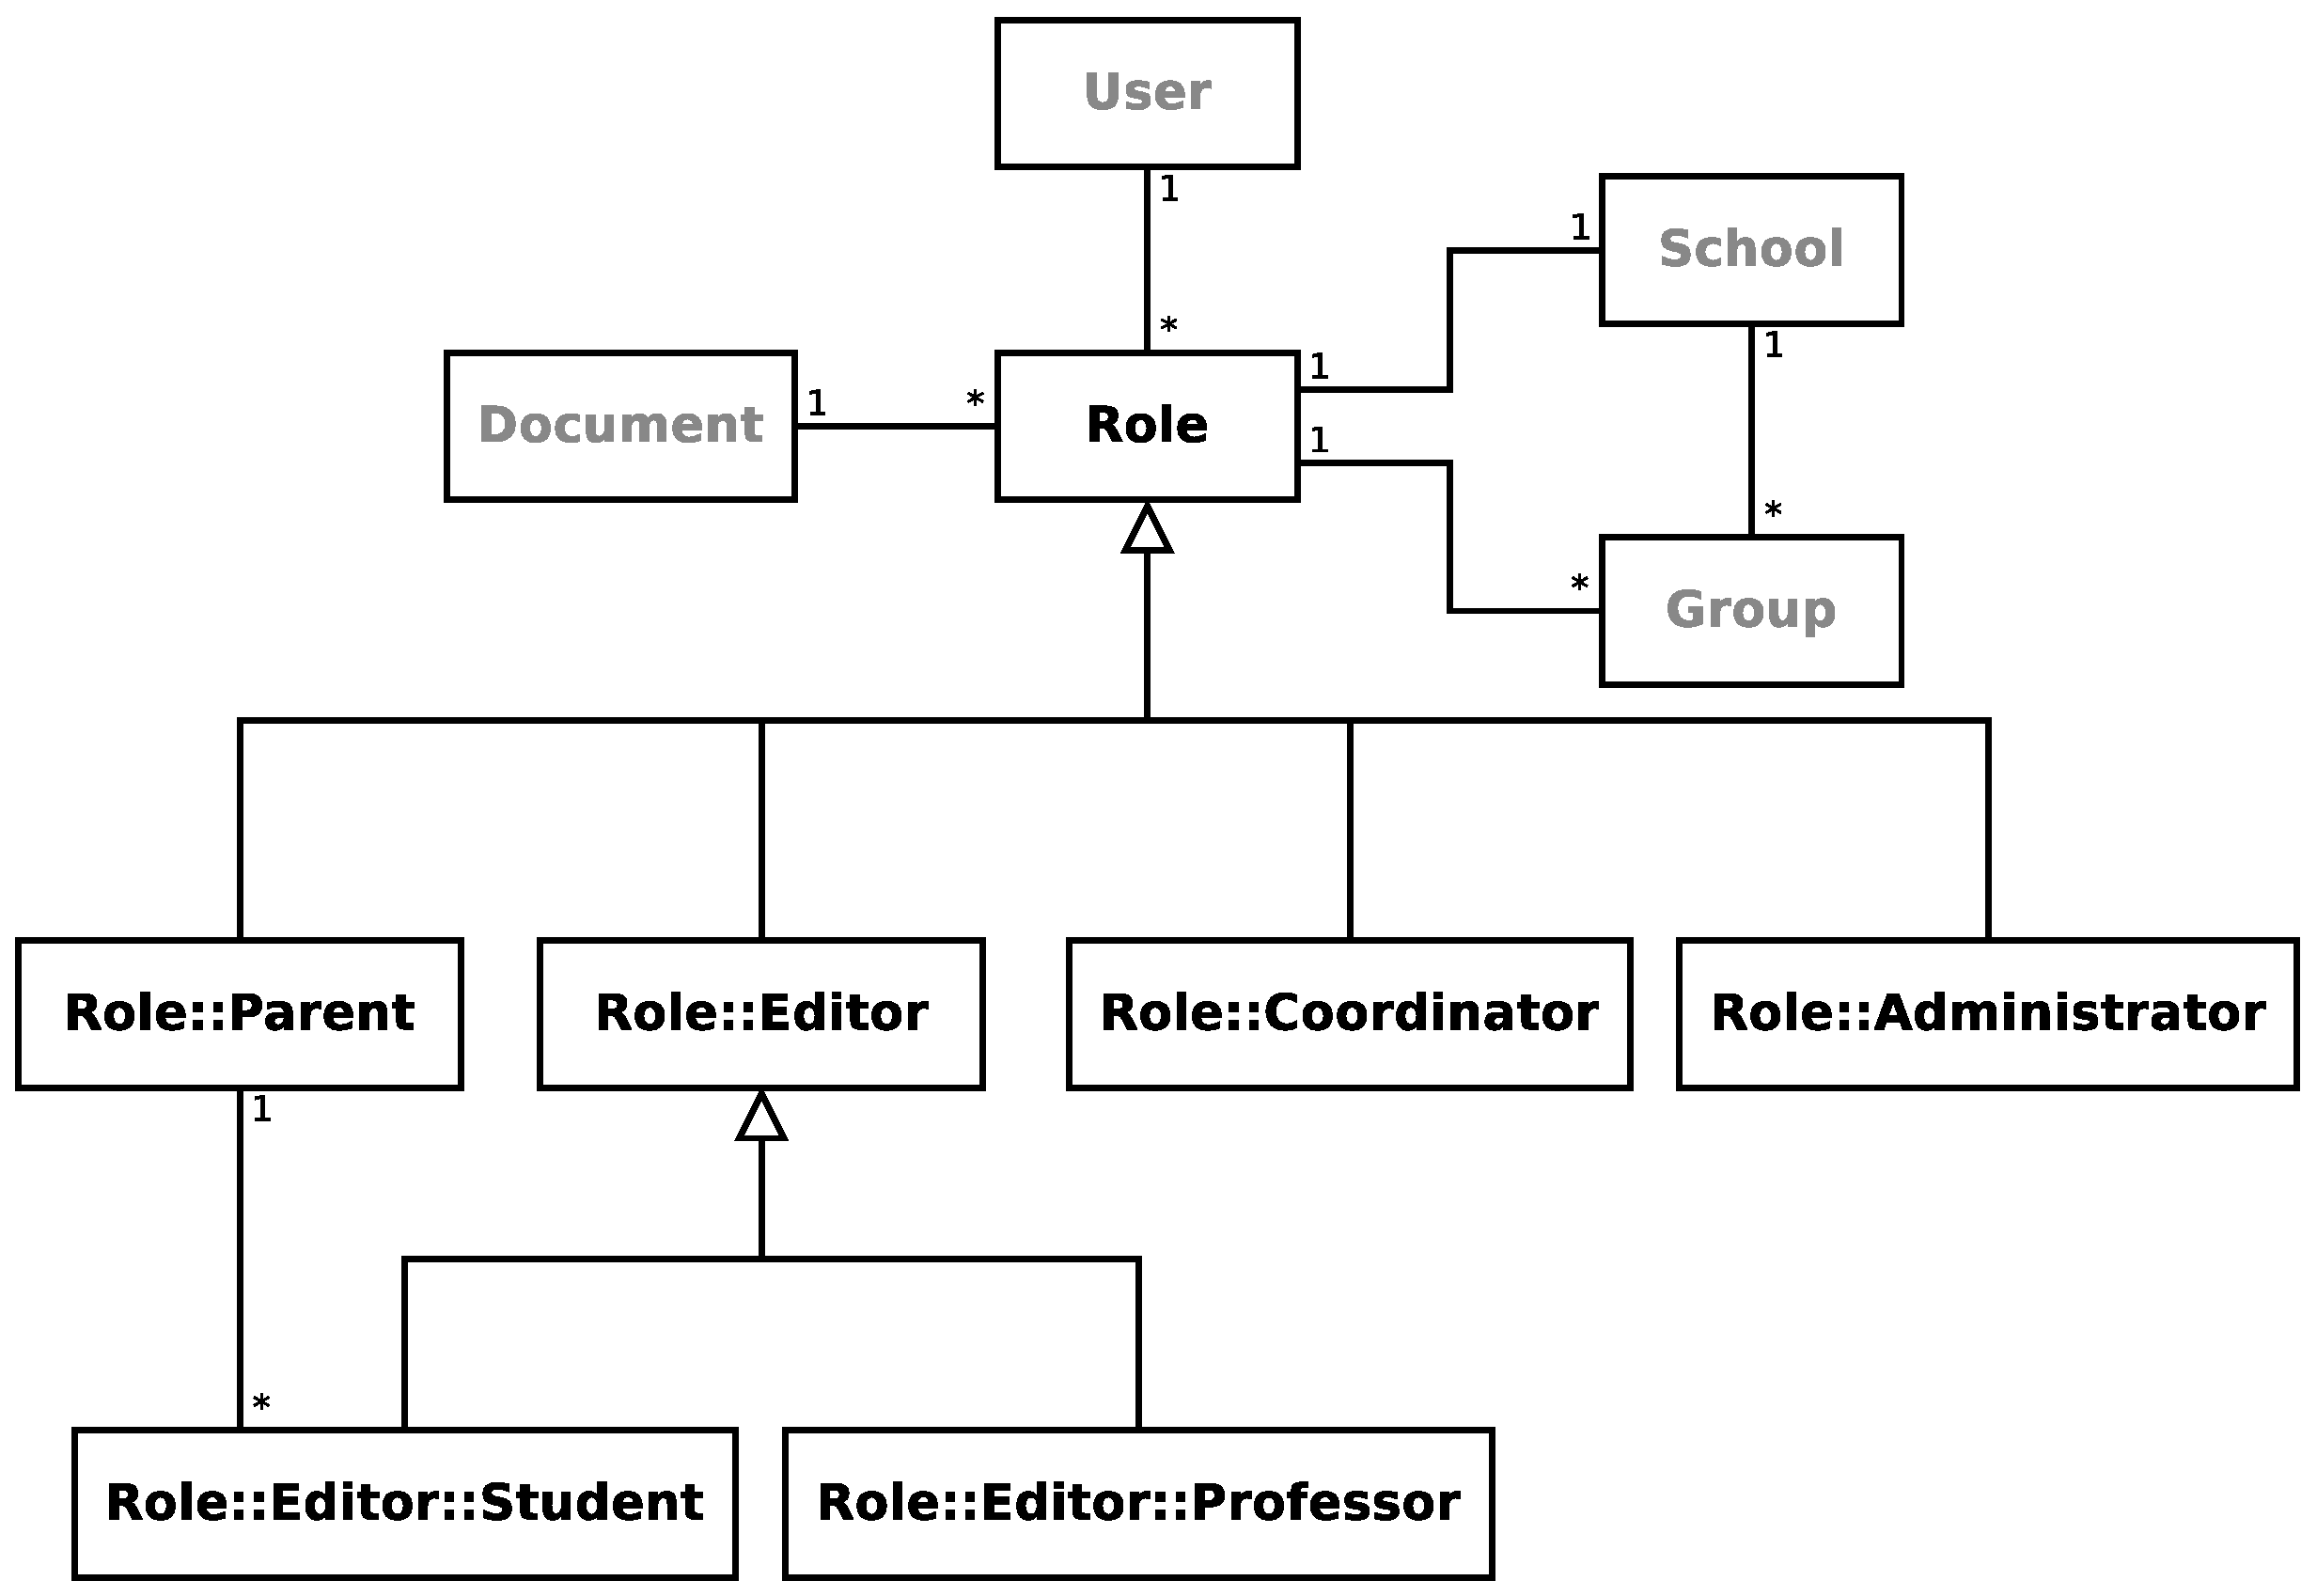
\includegraphics[width=0.4\textwidth]{figures/user_roles_current}}
  \caption{Desenho actual dos Papéis dos Utilizadores.}
  \label{fig:user_roles_current}
\end{figure}

%By using the \textsc{Role Object} pattern, the roles are split into single classes, which allows capturing the key abstractions of each one individually. By flattening the hierarchy, it is now possible to develop roles individually, as well as have users associated with multiple roles without fear of rule clashing.

Com o uso do padrão \textsc{Role Object}, os papéis do utilizadores são separados em entidades singulares, o que permite que a definição das suas abstrações chave seja feita individualmente. Ao alisar a hierarquia, torna-se possível o desenvolvimento individual dos papéis, sem problemas de contradição de regras.

\begin{figure}[H]
  \centering{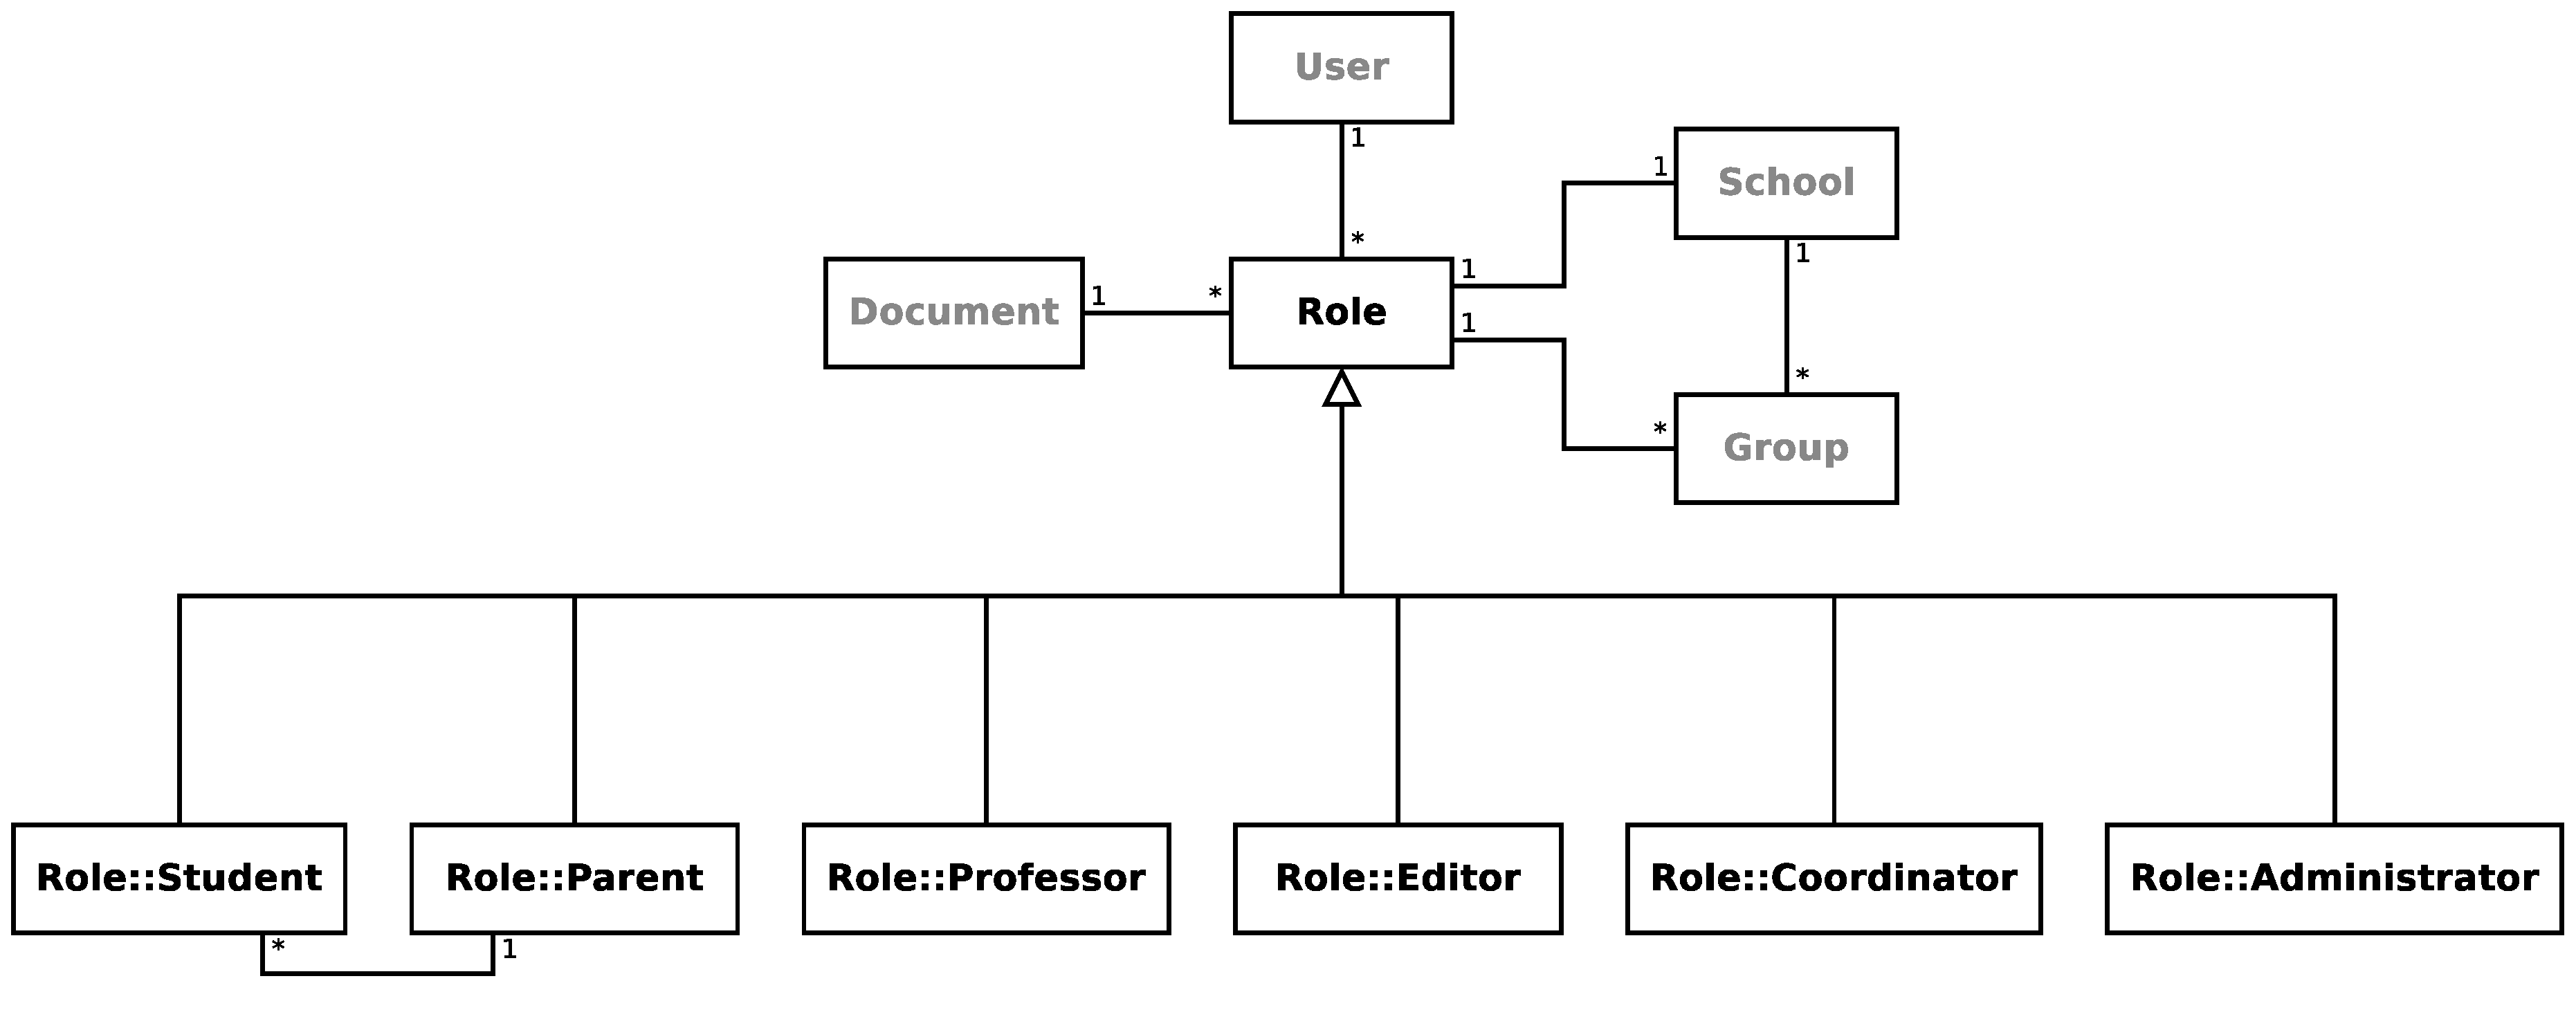
\includegraphics[width=0.4\textwidth]{figures/user_roles_conceptual}}
  \caption{Desenho conceptual dos Papéis dos Utilizadores.}
  \label{fig:user_roles_conceptual}
\end{figure}

\section{Rede Social}\label{sec:social_network}

%The current design for the escolinhas.pt social network is based on the relationships formed through the connections between users and their schools, groups, and other users, as depicted in Fig.~\ref{fig:social_network_current}. This allows the construction of a network where all the connections can be inferred dynamically and where an user can be identified towards another through these same connections. This model, however useful, offers a very small degree of variability.

O desenho actual da rede social da plataforma \emph{escolinhas.pt} assenta nas relações criadas através de ligações entre os utilizadores e as suas escolas, turmas e até mesmo outros utilizadores, como mostrado na Fig.~\ref{fig:social_network_current}. Isto permite a construção de uma rede onde todas as ligações pode ser inferidas dinamicamente e onde um utilizador pode ser perante outro através destas mesmas ligações. Apesar de útil, este modelo oferece um grau muito baixo de variabilidade.

\begin{figure}[H]
  \centering{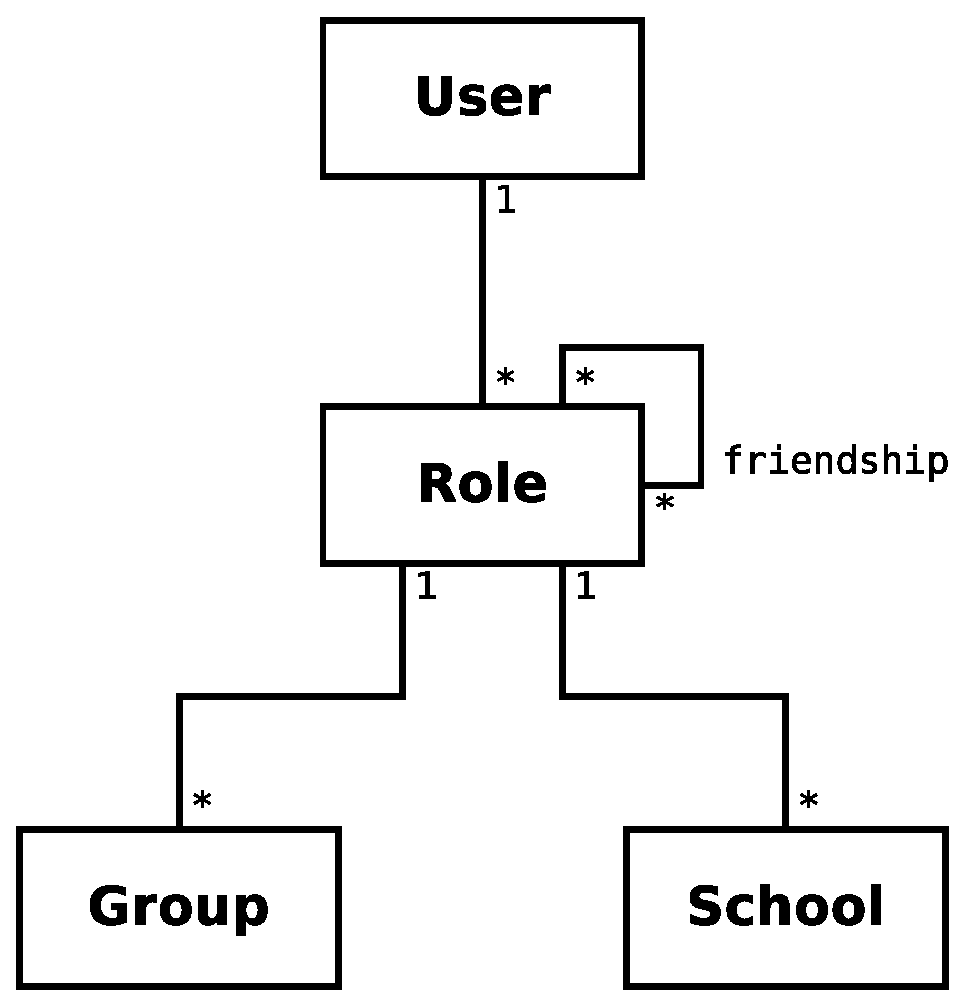
\includegraphics[width=35mm]{figures/social_network_current}}
  \caption{Desenho actual da Rede Social.}
  \label{fig:social_network_current}
\end{figure}

%The usage of the \textsc{Accountability} design pattern, by Martin Fowler~\cite{fowler_accountability} allows the creation of a relationship between two different entities in the system, with a third optional entity providing more information as to how they are connected.

O uso do padrão de desenho \textsc{Accountability}, por Martin Fowler~\cite{fowler_accountability} permite a criação de relações entre quaisquer duas entidades do sistema, com uma terceira entidade opcional que pode providenciar mais informações relativamente ao modo como as duas entidades originais estão ligadas.

\begin{figure}[H]
  \centering{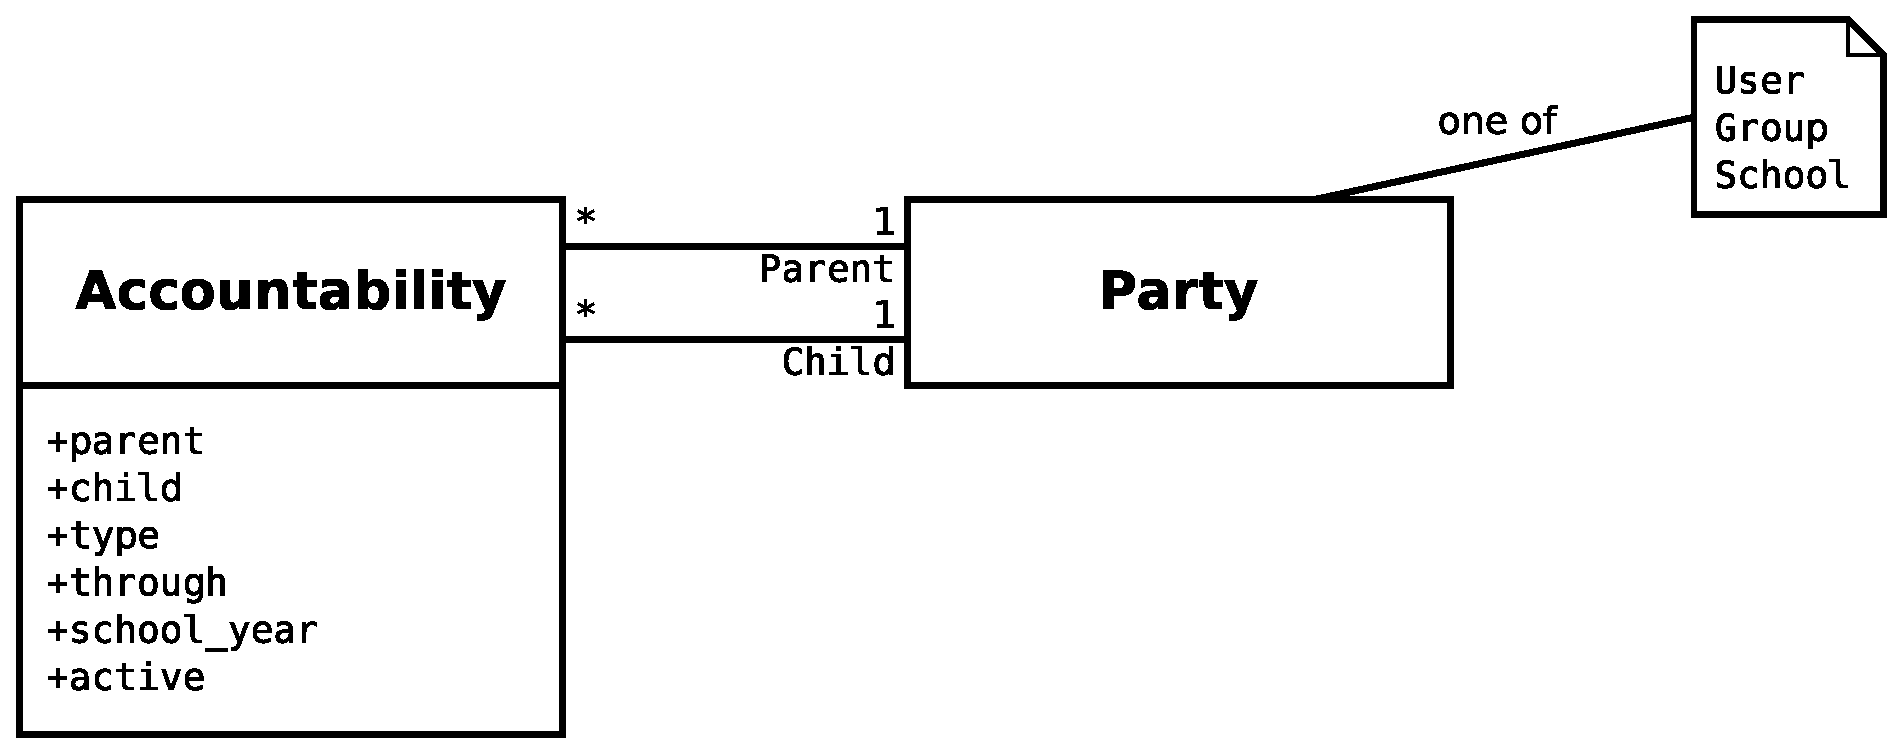
\includegraphics[width=0.4\textwidth]{figures/social_network_conceptual}}
  \caption{Desenho actual da Rede Social.}
  \label{fig:social_network_conceptual}
\end{figure}

\section{Editor de Documentos}\label{sec:document_editor}

%The existing document editor in \emph{escolinhas.pt} is one of the core components of the system and one of the used features. This being the case, and due to the constantly evolving nature of the product and the product itself, it is also one of the most modified parts of the system. The document editor infrastructure has to grow both in size and complexity every time a new type of block content is introduced --- represented by the gray entities in Fig.~\ref{fig:documents_current} --- by creating 

O editor de documentos presente no \emph{escolinhas.pt} é um dos componentes centrais do sistema e uma das funcionalidades mais usadas. Sendo este o caso, e devido à constante evolução da plataforma, é também um dos seus componentes mais modificados. A infrastrutura do editor cresce em tamanho e complexidade sempre que é necessário introduzir um novo tipo bloco --- representado pelas entidades a cinzento na Fig.~\ref{fig:documents_current} --- criando um novo Modelo, Controlador e Vistas, e duplicando toda a lógica presente de um bloco já existente.

\begin{figure}[H]
  \centering{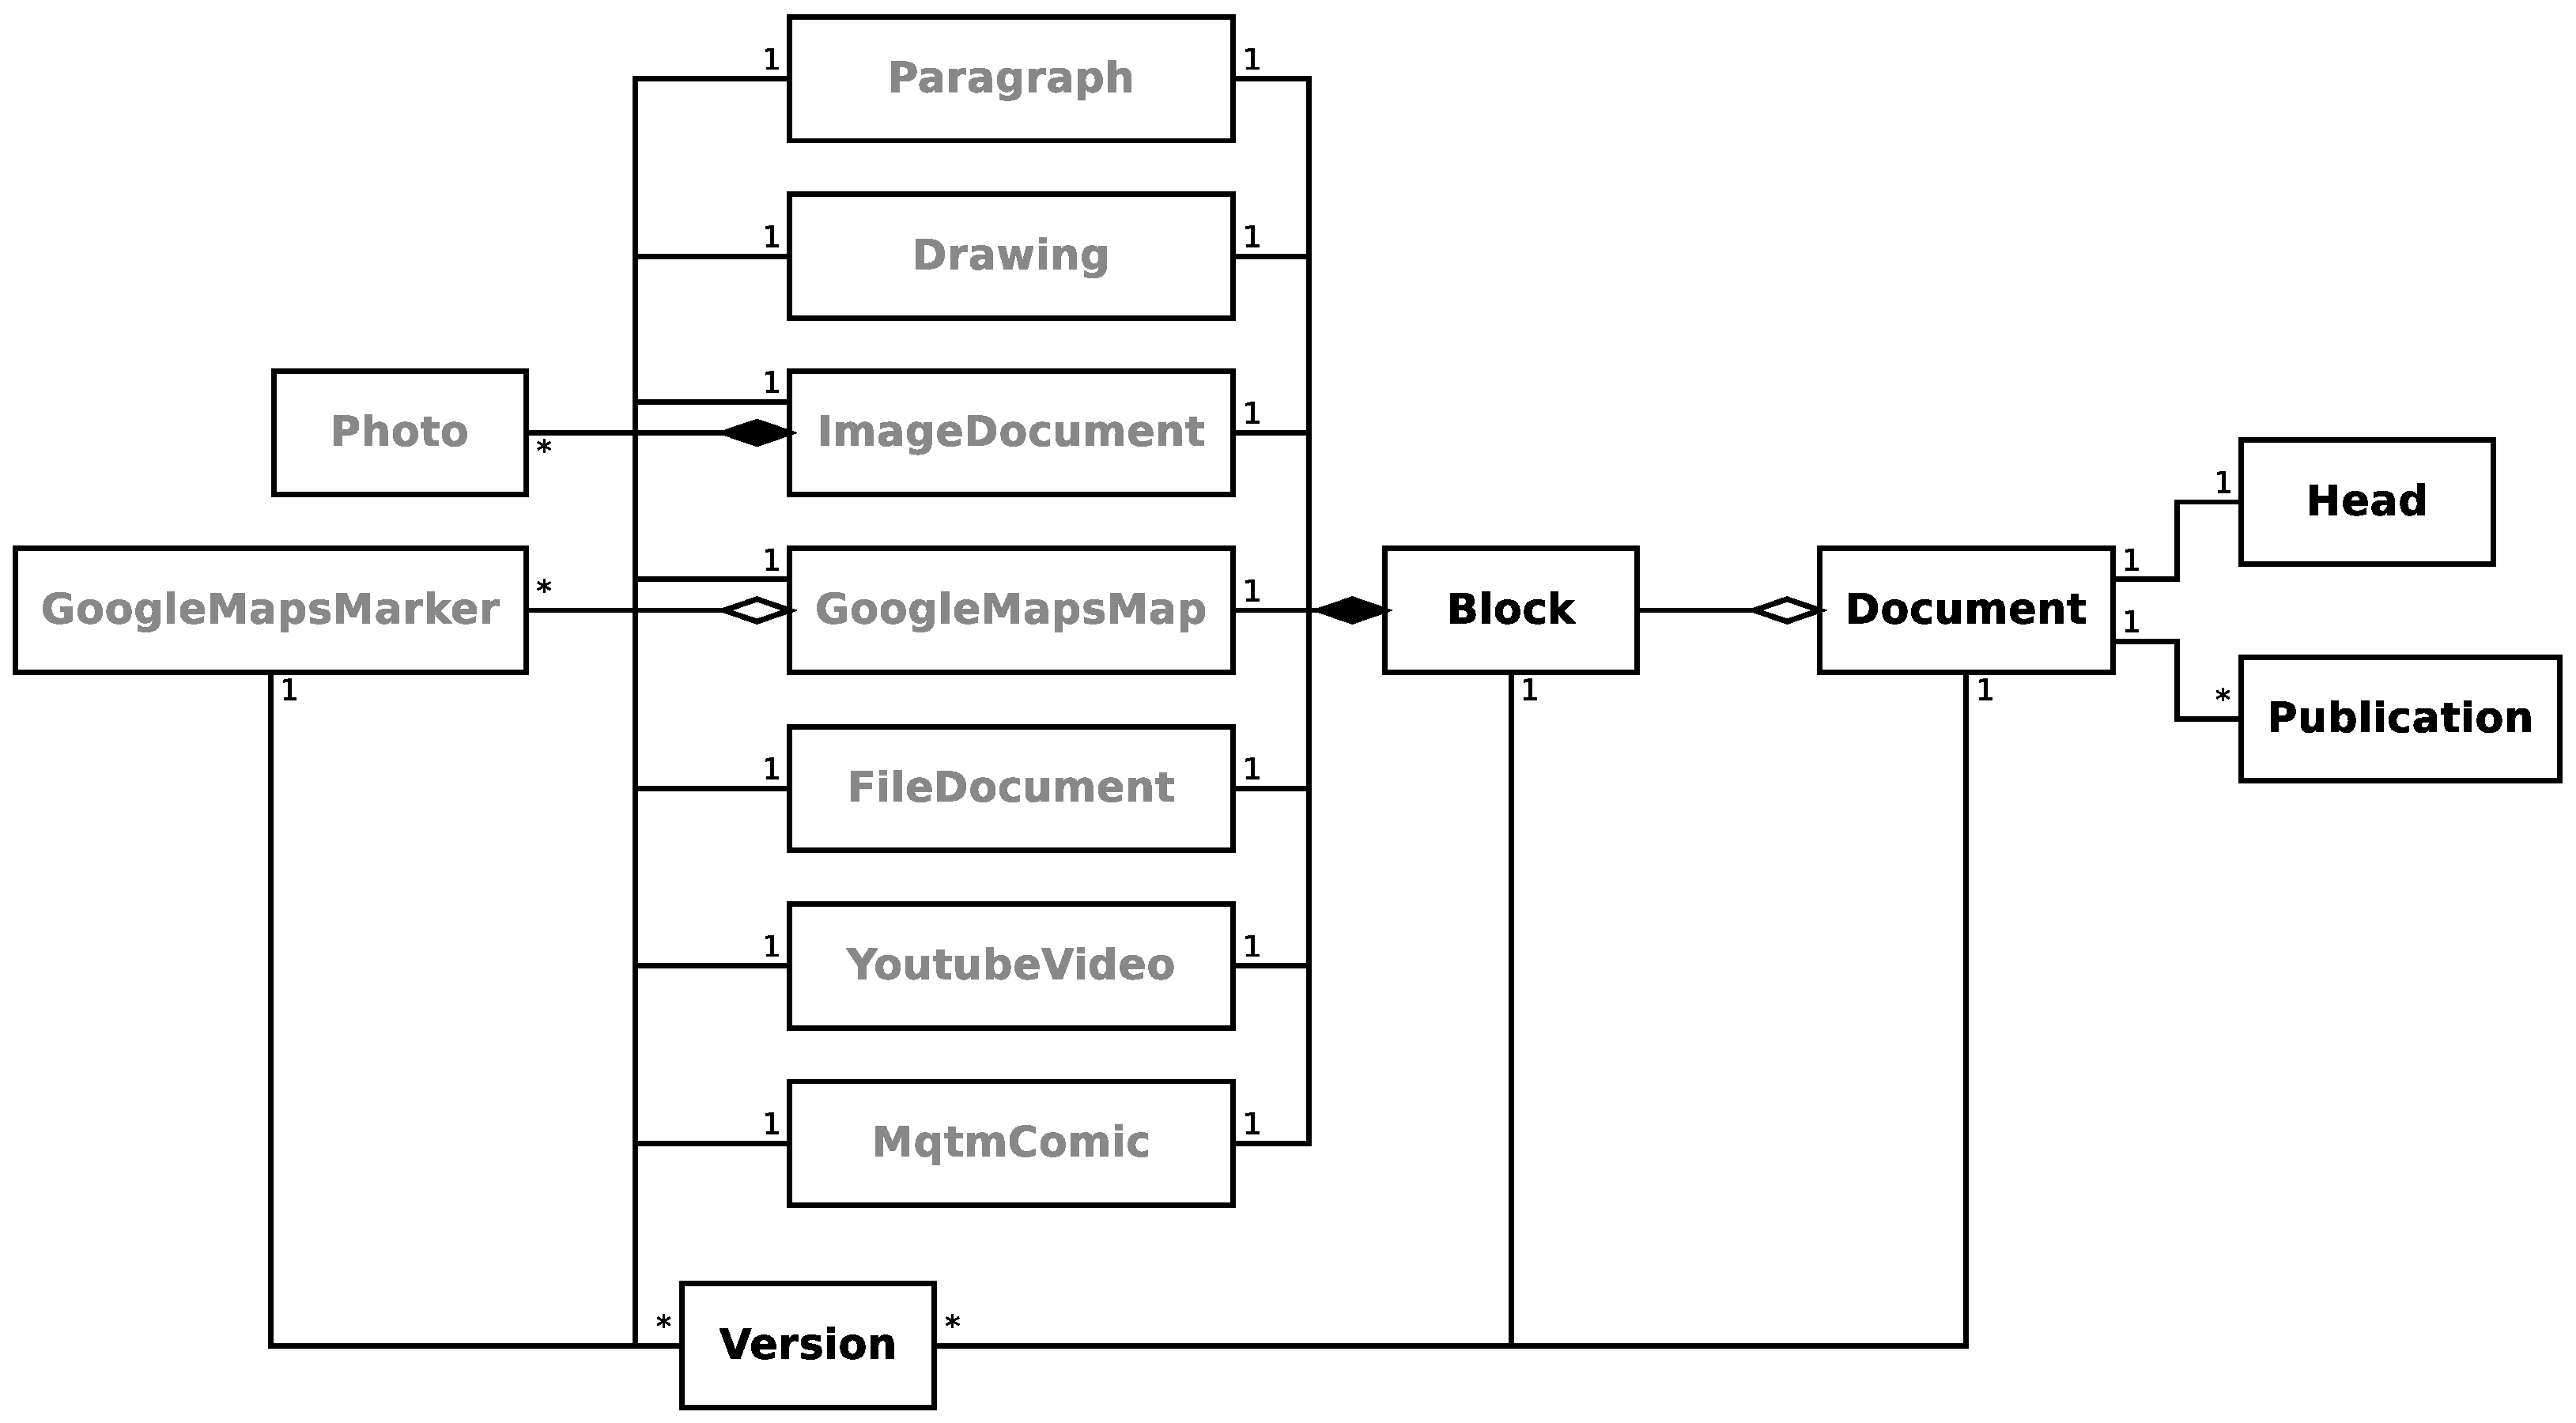
\includegraphics[width=0.4\textwidth]{figures/documents_current}}
  \caption{Desenho actual da infrastructura dos Documentos.}
  \label{fig:documents_current}
\end{figure}

%The solution devised for the \emph{Documents} infrastructure is, the simplest structure possible that makes everything work (as seen in Fig.~\ref{fig:documents_conceptual}). This is made possible by using a variant of the \textsc{Property} pattern~\cite{metadata_and_active_object_models} and the \textsc{System Memento}~\cite{patterns_data_and_metadata_evolution_in_aoms}

A solução desenvolvida para a infraestructura do editor de documentos passa por criar o desenho mais simples possível (tal como visto na Fig.~\ref{fig:documents_conceptual}). Isto é possível devido ao uso dos padrões de desenho \textsc{Property}~\cite{metadata_and_active_object_models} (variante) e \textsc{System Memento}~\cite{patterns_data_and_metadata_evolution_in_aoms}

\begin{figure}[H]
  \centering{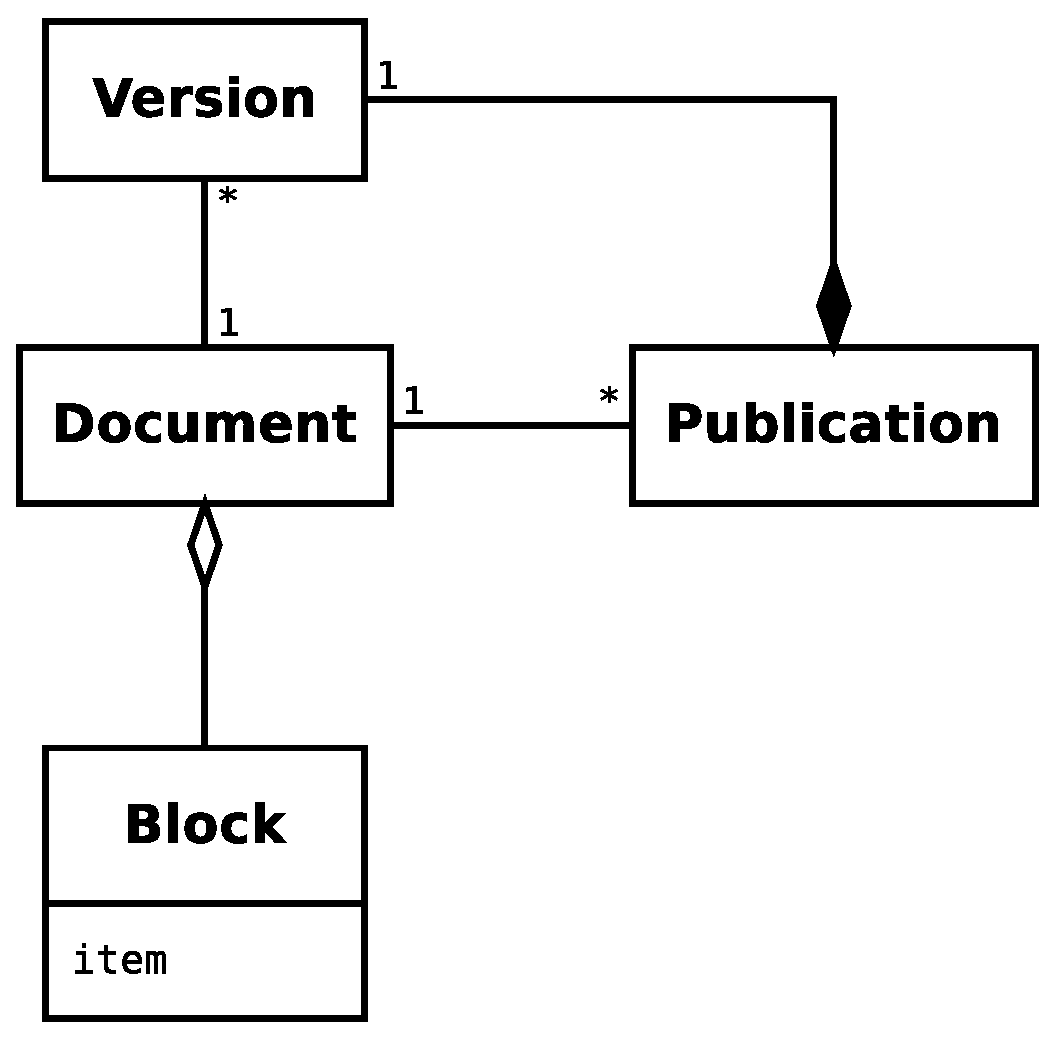
\includegraphics[width=25mm]{figures/documents_conceptual}}
  \caption{Desenho conceptual da infrastructura dos Documentos.}
  \label{fig:documents_conceptual}
\end{figure}

\section{Conclusion}\label{sec:conclusion}

%Despite being built with an MVC architecture, the Ruby On Rails framework is, using the right approach, capable of working with some architectural and design patterns --- present in AOM architectures --- not obviously connected with MVC and AR. The application of these patterns is capable of increasing the level of variability present in a common Rails application, and a harmonious integration with the Rails 2.3.x infrastructure --- especially the \textsc{ActiveRecord} engine --- is possible and works elegantly.

Apesar de ser usada para construir aplicações com arquitecturas baseadas em MVC, a framework \emph{Ruby On Rails} é, usando a abordagem correcta, capaz de conviver com alguns padrões arquitectónicos usados em arquitecturas AOM e não obviamente ligados ao MVC e \textsc{ActiveRecord}. A aplicação destes padrões é capaz de aumentar o nível de variabilidade existente numa aplição \emph{Rails} normal --- uma integração harmoniosa com a infraestructura providenciada pela framework \emph{Rails} 2.3.x --- especialmente o motor \textsc{ActiveRecord} --- é possível e funciona de forma elegante.

%It is also possible to conclude that the application of the appropriate design patterns is able to increase not only the variability and configurability needs of a specific part of an application, but also its performance, in some cases. However, this should not be taken as an universal truth, as it depends on a series of factors that may not be present in all implementations, such as a previous innapropriate design.

É também possível concluir que aplicação de padrões de desenho adequados é capaz de aumentar não só a variabilidade como a performance de um sistema, em alguns casos. No entanto, esta conclusão não deve ser tomada universalmente, já que depende de uma série de outros factores que poderão não estar presentes em todas as aplicações, tais como um desenho inadequado.

%%English version: comment first, uncomment second
\bibliographystyle{unsrt-pt}  % numeric, unsorted refs
%\bibliographystyle{numeric}  % numeric, unsorted refs
\bibliography{article-pt}

\end{multicols}

\end{document}
